\documentclass[tikz,border=10pt]{standalone}
\usepackage{amsmath}
\usepackage{tikz}
\usetikzlibrary{positioning, arrows.meta, fit, backgrounds, calc}

\begin{document}
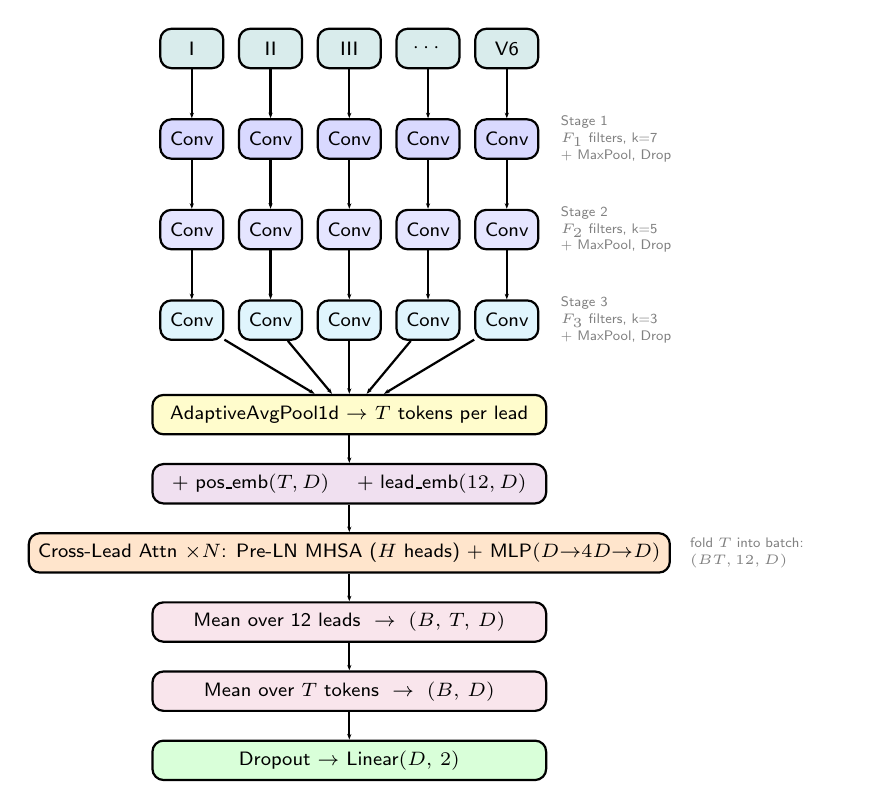
\begin{tikzpicture}[
    node distance=0.35cm,
    box/.style={draw, rounded corners, minimum height=0.5cm,
                font=\scriptsize\sffamily, align=center, thick},
    lead/.style={box, fill=teal!15, minimum width=0.8cm},
    conv/.style={box, fill=blue!15, minimum width=0.8cm},
    wide/.style={box, minimum width=5.0cm},
    attnbox/.style={wide, fill=orange!20},
    poolbox/.style={wide, fill=yellow!20},
    embbox/.style={wide, fill=violet!12},
    fusebox/.style={wide, fill=purple!10},
    outbox/.style={wide, fill=green!15},
    arrow/.style={-{Stealth[length=2pt]}, thick},
    lbl/.style={font=\tiny\sffamily, text=gray},
]

% ── Lead inputs ──────────────────────────────────────────────────────────
\foreach \i/\lead in {0/I, 1/II, 2/III, 3/{$\cdots$}, 4/V6} {
    \pgfmathsetmacro{\xpos}{-2 + \i * 1.0}
    \node[lead] (in\i) at (\xpos, 0) {\lead};
}

% ── Stage 1: k=7, F1 filters + MaxPool ───────────────────────────────────
\foreach \i in {0,1,2,3,4} {
    \pgfmathsetmacro{\xpos}{-2 + \i * 1.0}
    \node[conv] (s1\i) at (\xpos, -1.15) {Conv};
    \draw[arrow] (in\i) -- (s1\i);
}
\node[lbl, right=0.15cm of s14, text width=2.3cm]
    {Stage 1\\$F_1$ filters, k=7\\+ MaxPool, Drop};

% ── Stage 2: k=5, F2 filters + MaxPool ───────────────────────────────────
\foreach \i in {0,1,2,3,4} {
    \pgfmathsetmacro{\xpos}{-2 + \i * 1.0}
    \node[conv, fill=blue!10] (s2\i) at (\xpos, -2.30) {Conv};
    \draw[arrow] (s1\i) -- (s2\i);
}
\node[lbl, right=0.15cm of s24, text width=2.3cm]
    {Stage 2\\$F_2$ filters, k=5\\+ MaxPool, Drop};

% ── Stage 3: k=3, F3 filters + MaxPool ───────────────────────────────────
\foreach \i in {0,1,2,3,4} {
    \pgfmathsetmacro{\xpos}{-2 + \i * 1.0}
    \node[conv, fill=cyan!12] (s3\i) at (\xpos, -3.45) {Conv};
    \draw[arrow] (s2\i) -- (s3\i);
}
\node[lbl, right=0.15cm of s34, text width=2.3cm]
    {Stage 3\\$F_3$ filters, k=3\\+ MaxPool, Drop};

% ── AdaptiveAvgPool → T tokens per lead ──────────────────────────────────
\node[poolbox] (pool) at (0, -4.65)
    {AdaptiveAvgPool1d $\to$ $T$ tokens per lead};
\foreach \i in {0,1,2,3,4} { \draw[arrow] (s3\i) -- (pool); }

% ── Position + Lead embeddings ────────────────────────────────────────────
\node[embbox, below=0.35cm of pool] (emb)
    {$+\;\text{pos\_emb}(T,D)$ \quad $+\;\text{lead\_emb}(12,D)$};
\draw[arrow] (pool) -- (emb);

% ── Cross-lead attention block(s) ─────────────────────────────────────────
\node[attnbox, below=0.35cm of emb] (attn)
    {Cross-Lead Attn $\times N$: Pre-LN MHSA ($H$ heads) + MLP$(D{\to}4D{\to}D)$};
\draw[arrow] (emb) -- (attn);
\node[lbl, right=0.12cm of attn, text width=2.0cm]
    {fold $T$ into batch:\\$(BT,12,D)$};

% ── Mean over leads ───────────────────────────────────────────────────────
\node[fusebox, below=0.35cm of attn] (meanL)
    {Mean over 12 leads $\;\to\;(B,\,T,\,D)$};
\draw[arrow] (attn) -- (meanL);

% ── Mean over tokens ──────────────────────────────────────────────────────
\node[fusebox, below=0.35cm of meanL] (meanT)
    {Mean over $T$ tokens $\;\to\;(B,\,D)$};
\draw[arrow] (meanL) -- (meanT);

% ── Head ─────────────────────────────────────────────────────────────────
\node[outbox, below=0.35cm of meanT] (head)
    {Dropout $\to$ Linear$(D,\,2)$};
\draw[arrow] (meanT) -- (head);

\end{tikzpicture}
\end{document}
